\documentclass[10pt,journal,compsoc]{IEEEtran}
\usepackage[T1]{fontenc}
\usepackage{amsmath,amssymb,amsthm}
\usepackage{graphicx,booktabs,array}
\usepackage{listings}
\usepackage{url}
\usepackage[hidelinks]{hyperref}
\usepackage{cite}
\newtheorem{proposition}{Proposition}
\newcommand{\tool}{TraceSplit}
\lstset{basicstyle=\ttfamily\footnotesize,breaklines=true,columns=fullflexible,keepspaces=true,showstringspaces=false,frame=none,xleftmargin=3pt,xrightmargin=3pt}
\hyphenation{data-sets pre-pro-cess-ing coun-ter-fac-tu-al}
\begin{document}
\title{Checking Machine-Learning Workflows Through Execution Evidence}
\author{Ali~Al~Bataineh%
\IEEEcompsocitemizethanks{\IEEEcompsocthanksitem A. Al Bataineh is with Computer Information Science, Higher Colleges of Technology, Abu Dhabi, United Arab Emirates. E-mail: aalbataineh@hct.ac.ae. ORCID: 0000-0001-9530-7950.}}
\IEEEtitleabstractindextext{%
\begin{abstract}
Machine-learning (ML) experiments are programs, and a reported score depends on where transformations are fitted, which rows inform model selection, and whether held-out rows were used once. This article presents \tool{}, a closed workflow language for tabular classification and regression whose checker rejects protocol violations in the source, together with three forms of evidence about a completed run: a record checker that uses only the Python standard library, a standalone Python replay exported from the record, and fixed-partition counterfactual tests derived from a conditional held-out noninterference property. On 8 inputs and 5 seeds, all 40 workflows agree with their replays, all 600 altered records are rejected when the input file is supplied, and all 80 perturbations of the correct implementation preserve development state. An injected-fault study of 9 mechanisms and 330 faulty executions shows that the oracles cover different faults. Records that echo the declared protocol pass the checker, replay detects every fault that changes the compared outputs, and perturbation detects the faults that make development state depend on held-out values and no others. A matched comparison with the reference implementation of a recent workflow grammar on 12 violation families locates the boundary between a closed language and an embedded interface. The evidence mechanisms complement one another and should be combined rather than substituted.
\end{abstract}
\begin{IEEEkeywords}
Machine-learning software, domain-specific languages, data leakage, reproducibility, metamorphic testing, execution evidence.
\end{IEEEkeywords}}
\maketitle
\IEEEdisplaynontitleabstractindextext
\IEEEpeerreviewmaketitle

\section{Introduction}
\IEEEPARstart{M}{achine-learning} (ML) experiments are executable software. A reported score depends not only on an estimator but also on how observations are divided, where transformations are fitted, how candidates are selected, and which outputs are inspected during development. Leakage between development and held-out data compromises the interpretation of an apparently successful experiment and has been documented across scientific fields \cite{kapoor2023}. Static analysis of notebooks shows that software-engineering techniques can expose problematic information flows in ordinary data-science code \cite{yang2022,urban2025}. A language for experiments should therefore be judged by the behavior it makes explicit and checkable, not by how many lines it removes.

Consider a workflow that imputes missing values, standardizes predictors, compares three classifiers, and reports the best candidate's test score. Several distinct questions arise. Was preprocessing fitted on training rows? Were candidate decisions based on validation rather than test results? Does the exported program reproduce the recorded predictions? Could an apparently valid record have been generated by a different computation? A single successful run does not answer all of these questions, and neither does a readable record of that run.

Existing work addresses the first two questions at the source. Safe-DS provides a statically checked domain-specific language (DSL) for data science \cite{safeds2023}, Lale raises the abstraction level of pipeline construction \cite{lale2020}, a recent workflow grammar rejects leakage-prone calls at call time \cite{roth2026}, and lineage-based inspection explains how preprocessing changes a data distribution \cite{mlinspect2021}. The remaining questions concern the relation between a record and the computation it describes. A record written by the program that ran the experiment can agree with the declared protocol and with itself while describing a computation that did not take place.

This article treats the declared protocol, the saved record, a separately constructed numerical replay, and the response of a run to controlled changes in held-out data as four observation mechanisms with stated boundaries, and it measures what each mechanism detects. The implementation, \tool{}, supports supervised classification and regression on local comma-separated values (CSV) files. The contributions are the following.

First, \tool{} is a closed workflow language whose checker rejects protocol violations before execution and attaches source locations to a normalized execution plan. Each run produces a JavaScript Object Notation (JSON) record with hash-chained, source-linked events, a record checker that depends only on the Python standard library, a standalone Python export that reconstructs the numerical workflow without the language implementation, and a counterfactual harness that changes held-out values under frozen partitions.

Second, a conditional held-out noninterference proposition and a single-assessment proposition state exactly what the supported semantics guarantee. The first proposition supplies the oracle for the counterfactual tests.

Third, an evaluation on 8 inputs and 5 seeds covers 240 constructed programs, 40 numerical workflows with exported replays, 600 altered records, and 80 held-out perturbations. An injected-fault study applies 9 fault mechanisms to every workflow, producing 330 faulty executions, and examines each execution with the record checker, the replay, and the perturbation oracle. A matched comparison submits 12 protocol-violation families, expressed both as \tool{} programs and as call sequences for the mlw package that implements the workflow grammar of Roth \cite{roth2026,mlw2026}, to both tools on all inputs.

Fourth, the results separate the mechanisms. The record checker rejects every honest record of a scope violation and every altered record when the input file is supplied, but a faulty backend whose record echoes the declared protocol passes it. Replay detects every fault that changes a compared output and nothing else; its 14 misses on the preparation-scope fault are all classification workflows whose discrete predictions absorbed the altered scaling. Perturbation detects the faults in which development state depends on held-out values and none of the faults confined to training and validation rows. A replay exported from a record is faithful to the record rather than to the declared protocol. These observations support combining the mechanisms and give a concrete account of what each one establishes.

\section{Related Work and Research Position}
\subsection{Leakage detection and workflow restrictions}
Yang et al. analyze leakage in notebooks using static analysis and discuss process changes that prevent test information from influencing model development \cite{yang2022}. Urban et al. develop an abstract-interpretation-based analysis for leakage in ML programs \cite{urban2025}. Draoui et al. combine static slicing with structured language-model prompts to inspect training and evaluation paths in notebooks \cite{draoui2026}. These systems address existing programs in a considerably broader programming environment than the language evaluated here. \tool{} instead controls a small set of supported operations and does not claim equivalent coverage of arbitrary notebook code.

Safe-DS proposes a DSL with static checks for types, value ranges, data manipulation, and call order, and connects Python libraries through stubs \cite{safeds2023}. Lale provides consistent abstractions for ML pipelines and automated configuration \cite{lale2020}. The workflow grammar of Roth is the closest design. It arranges eight typed primitives in a directed acyclic graph, governs them by four constraints, and enforces a final assessment gate at call time \cite{roth2026}. Its Python reference implementation, mlw, registers partitions by content fingerprint when data are split, guards the fit, evaluate, and assess verbs against rows of the wrong role or of unknown origin, permits one assessment per held-out partition regardless of the model, and maintains an in-process hash-chained audit trail of verb invocations \cite{mlw2026}. The present article neither introduces the idea of checked ML workflows nor claims that terminal assessment is new. Its focus is the relation between the record of a restricted computation and additional tests of that computation, and Section~\ref{sec:comparison} measures where a closed language and an embedded interface differ on the same violations.

\subsection{Provenance and independently checked artifacts}
The W3C PROV data model distinguishes entities, activities, and agents when describing how data were produced \cite{prov2013}. The \tool{} record is a small, application-specific JSON format, not a PROV implementation. mlinspect extracts a dataflow graph from a pandas and scikit-learn pipeline and inspects the effect of preprocessing on data distributions \cite{mlinspect2021}. These precedents make it important to distinguish a readable history from a guarantee about the process that generated it.

Proof-carrying code separates an untrusted producer from a consumer that checks evidence against a safety policy \cite{necula1997}. \tool{} does not implement proof-carrying code; its evidence consists of recorded events, partitions, predictions, statistics, and fingerprints rather than a proof of the numerical computation. Translation validation checks an individual translation against a semantic relation \cite{pnueli1998}. The Python replay in this study is fixed-input differential testing, and agreement on the recorded inputs does not establish semantic equivalence for all programs.

\subsection{Testing when exact outputs are insufficient}
Metamorphic testing checks relations between executions when an exact output oracle is difficult to specify \cite{segura2016}. Here the relation concerns development state. For fixed partitions and schema, changing held-out values must not change training-derived preprocessing, fitted candidates, validation scores, or the selected candidate. Test-set noninterference is an established way of explaining leakage \cite{yang2022}; the contribution is an executable, restricted form of that relation used alongside record and replay checks. Model selection also has statistical limits that no workflow grammar removes, because optimizing choices against a finite evaluation sample introduces selection bias \cite{cawley2010}. The language enforces a local protocol within one run, not the validity of an entire research process.

\section{Language and Execution Design}
\subsection{Scope and intended use}
Version 0.1.0 supports supervised classification and regression on local CSV files. Classification estimators are logistic regression, a random forest, and a decision tree. Regression substitutes ridge regression for logistic regression. Numeric imputation, optional standardization, categorical imputation, and one-hot encoding are built into a single preparation operation. The numerical backend is scikit-learn \cite{sklearn2011}.

The language excludes arbitrary Python, general loops, user-defined functions, neural networks, cross-validation, and a general search procedure. This is a design boundary. A finite, explicit candidate list keeps the selection protocol inspectable. All candidates are trained on the same training partition, each is evaluated once on validation, and the winner is assessed once on test without refitting on training plus validation.

Listing~\ref{lst:iris} gives an executable two-candidate example. The experimental programs add a decision tree as a third candidate. The preparation command names its fitting role explicitly. Candidate evaluation and final assessment use different commands, so that an error message can identify a role violation rather than infer intent.

\begin{lstlisting}[caption={A complete classification workflow.},label={lst:iris},float=t]
read "datasets/iris.csv"
predict "target" as classification
split stratified train 60% validation 20% test 20% seed 42
prepare numeric median scale standard categorical most_frequent on train
train linear logistic C=1 on train
evaluate linear on validation
train forest forest trees=40 depth=6 on train
evaluate forest on validation
select best by accuracy
assess best on test
explain
\end{lstlisting}

\subsection{Parsing and semantic checks}
A Lark grammar recognizes statements and retains their source lines. The checker walks the parsed program, tracking the workflow phase and the sets of trained and evaluated candidates. A valid program has one read, one target declaration, one split, one preparation, one selection, and one assessment. Optional dropped columns occur before the split. Training and validation evaluation can be interleaved, provided that a candidate is trained before its evaluation and every declared candidate is evaluated before selection.

The checker rejects unsupported tasks, algorithms, metrics, parameters, and role combinations. Percentages are checked with decimal arithmetic and must be positive and sum to 100. Model names must be distinct. Seeds are bounded unsigned 32-bit integers. A program without terminal assessment is incomplete. After assessment, the only permitted statement is one optional request for an explanation.

The output is an immutable serialized plan containing commands, parameters, source locations, and source text. The execution application programming interface (API) accepts plans created by the checker. An internal validation marker prevents accidental execution of an arbitrary plan object through the normal API; it is not an unforgeable capability against a caller with access to Python internals.

\subsection{Partitions and feature preparation}
The supported partition strategies are random, stratified, grouped, and temporal. Random and stratified strategies use a seeded two-stage split. Grouped splitting assigns complete groups, so the declared percentages concern group counts. Temporal splitting orders observations by a declared numeric or date-time key and rejects equal keys crossing partition boundaries. The target, explicitly dropped columns, and the grouping or temporal metadata column cannot be predictors.

Preparation infers numeric and categorical column roles from the parsed data, then fits imputation, scaling, and encoding on training rows. Unknown categories map to an all-zero encoded vector. Dataset size, candidate count, and dense encoding size are bounded so that local review remains practical.

The distinction between data access and fitted dependence is essential. CSV parsing, input validation, stratification, grouping, and temporal ordering can inspect the full input, and a held-out value that changes type inference or invalidates the file can change acceptance. The invariant developed in Section~\ref{sec:semantics} therefore fixes the partition and schema and assumes that both inputs are accepted.

\subsection{Execution evidence and explanations}
Each successful run produces a JSON evidence record, a held-out prediction file, and a textual explanation. The record contains the normalized plan, a dataset fingerprint, zero-based row partitions, the predictor schema, fitted preprocessing state, model-state fingerprints, candidate validation predictions, final predictions, metrics, source-linked events, and environment information. Events identify split construction, preparation fitting, transformations, estimator fitting, validation evaluation, selection, and final assessment.

A hash chain links the recorded events, and hashes connect predictions and recorded states to their summaries. These are unkeyed SHA-256 consistency checks. They are not signatures, trusted timestamps, or attestations; a party that can change the record can recompute its hashes. The explanation is produced from saved execution fields. It reports row counts, fitted roles, candidate scores, selection, and source lines.

\section{Semantics and Evidence Boundaries}\label{sec:semantics}
\subsection{A restricted development-state model}
Let $D=(X,y)$ be an accepted input with fixed schema $S$ and fixed disjoint row partition $P=(T,V,H)$, where $T$, $V$, and $H$ denote the training, validation, and held-out test rows. Let $s$ include all declared seeds and fixed configuration values. The supported development computation is
\begin{align}
 \theta &= \operatorname{FitPrep}(X_T;S), \label{eq:prep}\\
 M_i &= \operatorname{Fit}_i(g_\theta(X_T),y_T;s),\quad i=1,\ldots,k, \label{eq:fit}\\
 v_i &= m\bigl(y_V,M_i(g_\theta(X_V))\bigr), \label{eq:val}\\
 i^* &= \operatorname{firstargmax}_{1\le i\le k}\,\sigma v_i. \label{eq:select}
\end{align}
Here $g_\theta$ is the fitted preprocessing transformation, $k$ is the number of declared candidates, $m$ is the declared selection metric, and the direction $\sigma$ is $-1$ for the root mean squared error (RMSE) and the mean absolute error (MAE) and $+1$ for the other supported metrics. The first maximizing candidate in declaration order wins a tie. Final assessment computes metrics from $M_{i^*}(g_\theta(X_H))$ and $y_H$ without refitting. Development state is
\begin{equation}
 A(D;P,S,s)=(\theta,M_1,\ldots,M_k,v_1,\ldots,v_k,i^*). \label{eq:state}
\end{equation}
The implementation observes preprocessing values, estimator-state fingerprints, validation metrics, and the winner as finite representations of this state.

\begin{proposition}[Conditional held-out noninterference]\label{prop:noninterference}
For deterministic supported operations under fixed versions and execution settings, suppose $D$ and $D'$ are both accepted, have the same $P$, $S$, and $s$, and agree on $T\cup V$. Then $A(D;P,S,s)=A(D';P,S,s)$.
\end{proposition}
\begin{proof}
Equation~\eqref{eq:prep} uses the same training predictors and schema, so it produces the same $\theta$. Equation~\eqref{eq:fit} then receives the same transformed training values, labels, configurations, and seeds for each candidate, producing the same $M_i$. The arguments of \eqref{eq:val} are unchanged, so the $v_i$ are equal. The same ordered scores and tie rule in \eqref{eq:select} yield the same winner. No held-out value is an argument of these development operations.
\end{proof}

This proposition is a property of the stated computation, not a machine-checked proof of the Python implementation or its dependencies. Its fixed-partition condition is substantive, because stratification can use held-out labels when partitions are first constructed. The counterfactual experiment therefore freezes row assignments and changes only values after that assignment has been established.

\begin{proposition}[Single terminal assessment]\label{prop:terminal}
Every accepted source program contains exactly one assessment statement, and no fitted or selection operation follows it within that program.
\end{proposition}
\begin{proof}
The checker accepts a completed program only in the assessed state. The sole transition into that state is assessment from the selected state. Once assessed, only one optional explanation is permitted; a second assessment or any training, preparation, evaluation, split, or selection command is rejected. Thus acceptance implies one assessment and excludes a later development operation.
\end{proof}

This source-level property does not prevent repeated execution of modified programs or external modification of the backend.

\subsection{A standard-library record checker}
The checker accepts an evidence record and, optionally, its CSV input. It checks the normalized protocol, source fingerprint, partition disjointness and exhaustive coverage, source-line references, allowed event sequence, candidate names, fitting roles, state and prediction fingerprints, selection consistency with the recorded validation scores, and terminal assessment. With the input file, it also verifies the data fingerprint, grouping or temporal constraints, excluded columns, and the reported metrics, which it recomputes from saved predictions and observed labels with its own arithmetic.

The checker can be executed with Python's site-package loading disabled. It does not import NumPy, pandas, scikit-learn, Lark, or the execution engine, so a record can be inspected without installing the ML stack. A successful check means that the supplied objects satisfy these record-level constraints. It does not prove that a specific estimator was fitted, that the supplied predictions came from that estimator, or that the source was interpreted honestly; in particular, the checker validates the normalized protocol and line metadata but does not reparse the original source.

\subsection{Fixed-input Python replay}
The exporter emits a standalone Python script, the exact CSV, the frozen row assignments, and the source workflow. The script reconstructs preprocessing, candidate fitting, scoring, and deterministic selection without importing \tool{}, using a separately assembled scikit-learn pipeline and an explicit array-based winner selection. The same backend libraries remain shared, so a backend defect can affect both paths.

Replay comparison checks the selected candidate, every candidate's validation metrics and predictions, and the selected candidate's test metrics and predictions, with absolute and relative tolerances of $10^{-10}$. Reusing frozen partitions and schema removes partition generation and schema inference from what this comparison tests.

\subsection{Records that echo the protocol}\label{sec:echo}
Suppose a faulty implementation fits the imputer and scaler on $T\cup V\cup H$ but records $T$ as the preparation-fitting scope. It can still record internally matching state fingerprints, predictions, scores, and event hashes, and given those predictions and the original CSV a checker recomputes the same scores. A record-level acceptance decision is therefore compatible with the wrong fitting procedure.

The evaluation generalizes this observation. For each injected fault, two records are produced. The honest record describes the rows that the faulty computation actually used. The echo record keeps the roles and row sets that the declared protocol prescribes and carries the numerical outputs of the faulty computation, with every dependent hash recomputed. The echo record models a backend that logs its intended protocol rather than its computation; it is not a model of an adversary who also fabricates counterfactual outputs and state fingerprints, and no mechanism in this article is claimed to resist that adversary.

\section{Evaluation Method}
\subsection{Questions and inputs}
The evaluation asks five research questions (RQs). RQ1 concerns conformance of the source checker and agreement with the standalone replay. RQ2 concerns the additional information obtained by providing the original CSV to the record checker. RQ3 concerns which injected faults each of the three evidence mechanisms detects. RQ4 concerns how the closed language and the embedded mlw interface decide the same protocol violations. RQ5 concerns the in-process overhead of source compilation relative to execution of an already compiled plan.

Table~\ref{tab:data} describes the 8 inputs. The five real datasets are small examples distributed with scikit-learn, whose documentation states that they are often too small to represent real-world learning tasks \cite{sklearndata}. Diabetes is loaded without the loader's default global scaling, so that fitted normalization is not inherited from outside the experiment \cite{sklearndiabetes}. The mixed fixture combines numeric predictors, two categorical columns, and missing values. The grouped fixture contains 60 groups of ten observations; the group column is excluded from predictors. The temporal fixture adds an ordered time key that is also excluded. The generator, exact CSV files, and hashes are distributed with the artifact.

\begin{table}[t]
\caption{Inputs used in the numerical evaluation. Rows is the number of observations; Features is the number of predictor columns, excluding the target and any split metadata column; Split is the declared partition strategy.}
\label{tab:data}\centering\footnotesize
\begin{tabular}{lrrll}\toprule
Input & Rows & Features & Task & Split\\\midrule
Iris & 150 & 4 & Class. & Stratified\\
Wine & 178 & 13 & Class. & Stratified\\
Breast cancer & 569 & 30 & Class. & Stratified\\
Digits & 1797 & 64 & Class. & Stratified\\
Diabetes & 442 & 10 & Regr. & Random\\
Mixed fixture & 800 & 14 & Class. & Stratified\\
Grouped fixture & 600 & 8 & Class. & Grouped\\
Temporal fixture & 600 & 8 & Regr. & Temporal\\
\bottomrule
\end{tabular}
\end{table}

Each input is evaluated at seeds 0, 1, 7, 42, 2026. Programs specify 60/20/20 training, validation, and test proportions, median numeric imputation, standard scaling, and most-frequent categorical imputation. Classification compares logistic regression ($C=1$), a 40-tree forest with maximum depth 6, and a decision tree of depth 5; regression substitutes ridge regression ($\alpha=1$). Selection uses accuracy for classification and RMSE for regression. This yields 40 workflows and 120 candidate fits per numerical execution path. Because temporal splitting is deterministic, the seed affects only the forest in the temporal workflows.

\subsection{Conformance corpus and altered records}
The conformance corpus contains 48 valid programs, formed from eight templates, three numeric imputation methods, and two scaling settings, and 192 invalid programs, produced by applying 24 mutation families to each template. The families include fitting on validation rows, preparation before splitting, premature selection, duplicate model names, invalid parameters, incompatible metrics, post-assessment fitting, and arbitrary Python syntax. The complete sources and expected labels are saved. They are constructed tests of the checker, not sampled developer errors.

For each numerical workflow, 15 record mutations alter one constraint each, yielding 600 altered records. The families target preparation, fit, evaluation, or assessment scope; partition coverage; source binding; candidate selection; metric consistency; prediction and state fingerprints; event order; and the dataset fingerprint. Mutations recompute chain hashes where appropriate so that detection is not attributed to a stale hash. Each record is checked with and without the original CSV.

\subsection{Counterfactual tests}
Two counterfactual executions of the correct implementation are constructed for each workflow. One perturbs only test predictors, applying $x'=11x+17$ to numeric held-out values and replacing categorical held-out values with a category absent from training. The other changes only test labels. The row partition is frozen, and the altered data must remain accepted under the same schema. The oracle compares preprocessing state, fitted-model fingerprints, validation scores, and the winner, the quantities of \eqref{eq:state}, and does not require final test predictions to remain equal. There are 80 such paired comparisons.

\subsection{Injected-fault matrix}\label{sec:faultmethod}
The fault study applies 9 mechanisms to every correct run. Seven change the backend computation: preparation fitted on all rows; preparation fitted on training and validation rows; estimators fitted on training and validation rows; test rows added to the training rows of every estimator; selection by the test score instead of the validation score; the winner refitted on training and validation rows before assessment; and estimators fitted with a seed other than the declared one. The eighth mechanism ignores the grouped or temporal rule and partitions rows at random while keeping the recorded strategy; it applies to the ten grouped and temporal workflows. The ninth mechanism changes the data rather than the backend by adding a predictor that is a noisy copy of the target; the engine then runs honestly on the altered file. In total there are 330 faulty executions.

Each faulty execution is examined by five observations. The honest record and the echo record of Section~\ref{sec:echo} are submitted to the record checker with the CSV, and the echo record also without it. A replay is exported from the echo record and compared with the record under the tolerances of the agreement test. The held-out feature perturbation is applied to the faulty backend under its frozen partitions, and the oracle of Proposition~\ref{prop:noninterference} is evaluated on the faulty development state. For the seven backend mechanisms and the partition mechanism, the faulty outputs are also compared with the correct run to establish whether the fault changed any compared output at all. For the data-level mechanism this comparison is undefined, because the correct run uses a different file.

\subsection{Matched comparison with an embedded interface}\label{sec:comparisonmethod}
The comparison expresses 12 protocol-violation families, together with the valid workflow, in both tools on all 8 inputs. For \tool{}, each family is a modification of the input's example program submitted to the checker. For mlw, each family is a sequence of calls to split, prepare, fit, evaluate, and assess on the same CSV, with the task declared explicitly, the scikit-learn engine selected, and the partition registry cleared before every case so that one case cannot influence another. Two families, adding test rows to the training rows and selecting by the test score, have no \tool{} syntax and are recorded as not expressible; in mlw they are expressed as fitting on a concatenated frame and as assessing two models on the same held-out partition. The mlw cases run in their own environment, because the package pins pandas below version 3; the versions and the raw outcomes are distributed with the artifact. A family counts as rejected when the tool raises an error before or during the offending call.

\subsection{Runtime procedure and execution environment}
The runtime comparison holds the engine and workflow constant. One path receives source text and compiles it before execution; the other receives a previously compiled plan. For 200, 2,000, 10,000 rows, 3 warm-up pairs precede 25 measured pairs, with the execution order alternating between pairs. Timing includes CSV loading, input checks, fitting, scoring, and in-memory evidence construction, and excludes interpreter startup, disk serialization, the external checker, and the replay. A seeded 10,000-resample percentile bootstrap of the paired median gives descriptive 95\% intervals, conditional on the measured machine and schedule.

All experiments were executed on the author's computer, a Windows 11 workstation with an Intel Core Ultra 7 155U processor (14 logical processors) running CPython 3.12.10 with NumPy 2.5.2, pandas 3.0.5, SciPy 1.18.1, scikit-learn 1.9.0, and Lark 1.3.1. Numerical library threads and forest workers were limited to one. Dependency versions, source snapshots, raw timing pairs, and run-level records accompany the article.

\section{Results}
\subsection{Conformance and numerical agreement (RQ1)}
All 48 valid constructed programs were accepted and all 192 invalid programs were rejected. Across the 40 numerical workflows, every standalone replay agreed with the language execution on the selected candidate, candidate validation predictions and metrics, and selected test predictions and metrics; the largest observed absolute difference was 0. Table~\ref{tab:outcomes} collects these outcomes together with the record and counterfactual tests.

\begin{table}[t]
\caption{Observed outcomes on the constructed evaluation. Each row gives the number of cases with the expected outcome over the number of cases. Counts describe this suite, not estimated real-world error rates.}
\label{tab:outcomes}\centering\footnotesize
\begin{tabular}{p{0.68\columnwidth}r}\toprule
Check & Outcome\\\midrule
Valid source programs accepted & 48/48\\
Invalid source programs rejected & 192/192\\
Standalone numerical replays agreeing & 40/40\\
Altered records rejected, CSV supplied & 600/600\\
Altered records rejected, no CSV & 520/600\\
Correct-engine counterfactual invariants preserved & 80/80\\\bottomrule
\end{tabular}
\end{table}

The automated implementation suite passed 296 tests with 94\% statement coverage over 711 statements. This suite overlaps the conformance corpus, so the counts are not independent observations. A subprocess smoke test separately executed the command-line interface, the standard-library checker, the exported Python script, and their comparison. Exact replay agreement shows that the two execution paths share the intended configuration on these inputs; both paths use scikit-learn and the same experimental specification, so a shared misunderstanding of the specification would survive this test.

\subsection{The contribution of the original CSV (RQ2)}
With the CSV supplied, the record checker rejected all 600 altered records. Without it, the checker rejected 520. The 80 additional rejections concern two mutation families across all 40 workflows: a changed dataset fingerprint and a coherently changed reported test metric. Without source data those fields are well formed; with source data the fingerprint can be checked and the metric recomputed from labels and saved predictions. The checker's median running time on a record with its CSV was 3.7 ms. This result identifies a specific information difference, not a general detection rate, and a consistent record with genuine labels can still describe a computation that did not occur.

\subsection{Injected faults and the three oracles (RQ3)}
Fig.~\ref{fig:faults} summarizes the 330 faulty executions. The record checker rejected every honest record of a fault that changed the rows used by preparation, fitting, selection, or assessment (240 of 240). It accepted every honest record of the undeclared-seed and partition-rule faults, because those records declare a protocol that differs from the source text and the checker does not reparse the source. Every echo record of the seven backend faults passed with and without the CSV, with one exception. For selection by the test score, the recomputed winner contradicted the recorded validation scores in 10 of 40 runs, exactly the runs in which the test-based winner differed from the validation-based winner, and those records were rejected with and without the CSV. The partition-rule fault was rejected in all 10 echo records when the CSV was supplied, because group identifiers or time keys crossed partition boundaries, and in none without it. The data-level fault passed every record check.

\begin{figure}[t]
\centering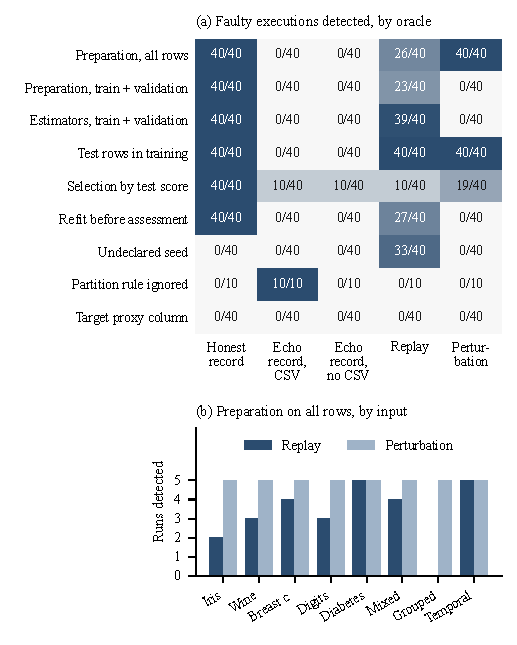
\includegraphics[width=\columnwidth]{figures/fault_matrix.pdf}
\caption{Injected-fault study. (a) Number of faulty executions detected by each observation, over the number of executions of that mechanism: rejection of the honest record with the CSV, rejection of the echo record with and without the CSV, disagreement between the echo record and its exported replay, and a change in development state under the held-out feature perturbation. Darker cells denote larger shares. The partition-rule mechanism applies to the ten grouped and temporal workflows. (b) For preparation fitted on all rows, the number of the five runs on each input in which replay and perturbation detected the fault.}
\label{fig:faults}
\end{figure}

Replay detected a fault whenever the fault changed a compared output. Across the 290 executions on unchanged data, the faulty outputs differed from the correct run in 208 executions, and replay disagreed with the echo record in 198. The two counts differ only for the partition-rule fault, where the exported replay freezes the recorded random partitions and reproduces the faulty computation in all 10 runs. A replay exported from a record is faithful to the record, not to the declared protocol. For the preparation-scope fault, replay detected 26 of 40 runs. Fig.~\ref{fig:faults}(b) shows that both regression inputs were detected in every run and that all 14 undetected runs are classification workflows, including all 5 runs on the grouped fixture. In those runs the altered standardization changed every fitted state, as the state fingerprints show, but left every compared label unchanged. Tree-based candidates are invariant to an affine rescaling applied uniformly to all rows, so on inputs without missing values the fault can surface only through the regularized linear candidate, and its discrete predictions were unchanged as well. Output-only comparison therefore misses a methodological fault whenever discrete predictions absorb the fault. The same mechanism explains the misses for preparation on training and validation rows (23 of 40), the refit before assessment (27 of 40), and the undeclared seed (33 of 40).

The perturbation oracle detected the faults in which development state depends on held-out values: preparation fitted on all rows in all 40 runs, test rows in training in all 40 runs, and selection by the test score in 19 of 40 runs, namely those in which the altered test values changed the test-based winner. It detected none of the 160 executions of the four faults confined to training and validation rows, none of the partition-rule executions, and none of the data-level executions, whereas replay detected 122 of those 160 confined executions. The two oracles therefore have nearly disjoint coverage. The record checker answers whether the recorded protocol is consistent, replay answers whether the numerical outputs follow from the recorded inputs, and the perturbation answers whether a prohibited dependency is exercised by the intervention. The target proxy column, a fault outside the protocol, passed all three, which locates the boundary of what any of these mechanisms can establish.

\subsection{Closed language and embedded interface (RQ4)}\label{sec:comparison}
Table~\ref{tab:comparison} reports the matched comparison. Both tools accepted the valid workflow on all 8 inputs. \tool{} rejected all ten expressible violation families on every input, and the remaining two families cannot be written. mlw 1.1.2 rejected seven families on every input, each with a partition error raised before the computation: fitting before any split or on test rows, fitting on a frame that concatenates training and test rows, evaluating on test rows, assessing on validation rows, assessing the same held-out rows twice, and assessing a second model on an already assessed partition. It accepted the other five families on every input: preprocessing before the split, preparation fitted on all rows, fit on validation rows, development operation after assessment, workflow without final assessment.

\begin{table}[t]
\caption{Matched protocol-violation families decided by the \tool{} checker and by the mlw package, as the number of inputs on which the family was rejected over the number of inputs. Families marked not expressible have no \tool{} syntax.}
\label{tab:comparison}\centering\footnotesize
\setlength{\tabcolsep}{4pt}
\begin{tabular}{p{0.56\columnwidth}cc}\toprule
Family & \tool{} & mlw\\\midrule
Valid workflow & 0/8 & 0/8\\
Fit before any split & 8/8 & 8/8\\
Preprocessing before the split & 8/8 & 0/8\\
Preparation fitted on all rows & 8/8 & 0/8\\
Fit on validation rows & 8/8 & 0/8\\
Fit on test rows & 8/8 & 8/8\\
Test rows added to training rows & not expressible & 8/8\\
Validation evaluation on test rows & 8/8 & 8/8\\
Selection by test score & not expressible & 8/8\\
Final assessment on validation rows & 8/8 & 8/8\\
Second assessment of the same test rows & 8/8 & 8/8\\
Development operation after assessment & 8/8 & 0/8\\
Workflow without final assessment & 8/8 & 0/8\\
\bottomrule
\end{tabular}
\end{table}

The differences follow from the two designs rather than from the quality of either implementation. mlw guards the data that enter its verbs, so preprocessing performed before the split is invisible to it, while in a closed language the same operation is an ordering or scope error in the source. mlw accepts validation rows in fit by documented design, does not require a final assessment, and in the probed version accepted a validation evaluation after the assessment; the closed language fixes training as the only fitting role and makes assessment terminal. Conversely, mlw rejected the two families that \tool{} cannot express, because the concatenated frame has no registered role and because the held-out partition is spent after its first assessment. Both tools decide protocol violations before any computation, and neither examines the computation inside the backend, which is the subject of RQ3.

\subsection{Observed frontend overhead (RQ5)}
Table~\ref{tab:runtime} reports the measured paired overhead of entering through the language frontend. The median paired differences were 0.339, 1.075, 0.076 ms for 200, 2,000, 10,000 rows, and all three bootstrap intervals include zero. The frontend performs extra work, but the largest absolute median difference of 1.075 ms is small relative to the execution itself, and scheduling noise dominates at the largest input. Fig.~\ref{fig:runtime} displays the raw paired distributions.

\begin{table}[t]
\caption{In-process execution time in milliseconds for the language path and the precompiled-plan path. Each row summarizes 25 measured pairs. Language and Plan API are median times, $\Delta$ is the median of the paired differences, and the interval is a 10,000-resample percentile bootstrap interval for that median.}
\label{tab:runtime}\centering\footnotesize
\begin{tabular}{rrrrl}\toprule
Rows & Language & Plan API & Paired $\Delta$ & 95\% interval\\\midrule
200 & 36.312 & 35.180 & 0.339 & [-0.884, 2.742]\\
2,000 & 64.732 & 64.213 & 1.075 & [-0.170, 2.928]\\
10,000 & 163.944 & 167.311 & 0.076 & [-3.207, 2.030]\\
\bottomrule
\end{tabular}
\end{table}

\begin{figure}[t]
\centering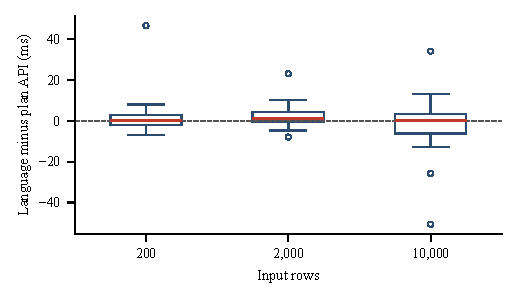
\includegraphics[width=\columnwidth]{figures/runtime_differences.pdf}
\caption{Language-minus-plan execution times for the 25 measured pairs at each input size. Boxes span the interquartile range, the center line marks the median, whiskers extend to 1.5 interquartile ranges, and circles are observations beyond the whiskers. The dashed line denotes equal measured times. Observations exclude interpreter startup and artifact serialization.}
\label{fig:runtime}
\end{figure}

\section{Reproducible Artifact and Reviewer Workflow}
The artifact includes the implementation, the exact grammar, the 8 input files and their source descriptions, the source programs, the configuration, the constructed mutation corpus, the fault and comparison scripts, the automated tests, the raw result files, and all 40 run directories. Each run directory holds an evidence record, a standalone replay, and its comparison. A smoke script gives a first installation check, and a single script rebuilds every reported number, table, and figure from the saved results.

A local browser application exposes program editing, results, explanations, the evidence record, and the exported Python through a standard-library Hypertext Transfer Protocol (HTTP) server bound to the loopback address. Its routes are covered by automated tests, and the application was exercised end to end in a browser on the author's computer. The reviewer can reproduce the central negative result directly. The supplied honest record of the preparation-scope fault fails the checker, while its echo counterpart passes. That accepted record is part of the expected outcome. The original code is provided under the MIT license with separate third-party notices.

\section{Limitations and Future Work}
The conformance cases, record mutations, and injected faults were designed for the supported constraints; their outcomes describe exercised behaviors, not completeness over all malformed programs or all leakage patterns. The specification, implementation, checker, exporter, and tests share one development process, and the record checker shares partition-semantics helpers with the engine, so correlated defects are possible. The held-out invariant is conditional on stable schema and fixed row assignments, and source-level role restrictions cannot identify target proxies, duplicated entities under different identifiers, or an unsuitable temporal boundary. The hash chain is evidence of consistency, not of honest execution, and an engine that fabricates both state and counterfactual outputs lies outside the evaluated threat model. Five inputs are small bundled datasets and three are generated fixtures; timing comes from one machine and one dependency set; and no participant study was conducted, so claims about comprehension or learning are outside the scope of this article.

The next evaluation would use independently curated workflow faults with in-scope and out-of-scope cases labeled before execution, and would extend the matched comparison to further tools on a common supported subset. Stronger authenticity would require a trusted boundary around the evidence producer, which additional hashing does not supply.

\section{Conclusion}
\tool{} implements a restricted language for tabular ML experiments with source-linked records, a standard-library evidence checker, standalone Python replay, and fixed-partition counterfactual tests. In the evaluated suite, 240 constructed programs received their expected decisions, 40 workflows matched their replays, 600 altered records were rejected with the input file, and 80 correct-engine perturbations preserved development state. The injected-fault study of 9 mechanisms and 330 executions shows where each mechanism stops. A record that echoes the declared protocol passes the checker; replay detects exactly the faults that change a compared output and is blind when discrete predictions absorb the fault; perturbation detects exactly the faults that make development state depend on held-out values. The matched comparison with mlw shows that a closed language removes some violations by construction and rejects the rest before execution, while an embedded interface cannot see computations outside its verbs. Record consistency, numerical agreement, and sensitivity to held-out information are three different properties, and a reviewer who wants all three must check all three.

\bibliographystyle{IEEEtran}
\bibliography{References}
\end{document}
